\documentclass[10pt]{article}
\usepackage{amsmath,amsthm,amssymb}
\usepackage{graphicx}
\graphicspath{{./images/}}
\begin{document}
\title{Various Technical Details}
\date{\vspace{-5ex}}
\author{Andrew Ott}


\maketitle


%%%%%%%%%%%%%%%%%%%
%Abstract
%%%%%%%%%%%%%%%%%%%
\section{Definitions}
Kullback-Leibler:
\begin{equation} \label{kl}
\mathrm{KL}(p(x)|| q(y)) = - \mathrm{E}_{p_(x) } [log\frac{q(y)}{q(x)}]
\end{equation}
Note: The Kullback-Leibler is non-negative.\\
The Variational Lower Bound, frequently called the evidence lower bound(ELBO):
\begin{equation}\label{Lower_Bound1}
\mathcal{L}(q)= -\mathrm{KL}(q(z|x)||p(x,z))
\end{equation}
A little algebra changes (\ref{Lower_Bound1})  into the following:

\begin{equation}\label{Lower_Bound2}
\mathcal{L}(q)= -\mathrm{KL}(q(z|x)||p(z)) + \mathrm{E}_{q_(z|x)} [log{p(x|z)}]
\end{equation}

This is the form used most frequently in the literature.  The KL term in (\ref{Lower_Bound2}) measures the difference between the variational posterior $p(z|x)$ and the prior $p(z)$.  The expectation in (\ref{Lower_Bound2}) is called the reconstruction error.  While the term is itself intractible, it lends itself to easy MC sampling by sampling some $z \sim q(z|x)$ then putting it into the log.  See (Kingma \& Welling, 2013) section 2.3 for more details.  In fact, a thorough understanding of this paper and its implementation will help you understand much of VAEs, as it is the paper that created the VAE, alongside (Rezende, et al., 2014).  I have included a fly-by summary of (Kingma \& Welling, 2013) in section 5 of this paper. 


\section{Background}
Variational Lower Bound Identity:
\begin{equation}\label{logp_Equality}
logp(x) = \mathcal{L}(q) + \mathrm{KL}(q(z|x)||p(z|x))		
\end{equation}
\begin{proof}
	\begin{align*}
		logp(x) &= \mathrm{E}_{q(z|x)}[logp(x)] \\
		&= \mathrm{E}_{q(z|x)}[logp(x,z) - logp(z|x)]\\
		&= \mathrm{E}_{q(z|x)}[(logp(x,z) - logq(z|x)) - (logp(z|x)- logq(z|x))]\\
		&= \mathrm{E}_{q(z|x)}[(logp(x,z) - logq(z|x))] - \mathrm{E}_{q(z|x)}[logp(z|x)- logq(z|x)]\\
		&= \mathcal{L}(q) + \mathrm{KL}(q(z|x)||p(z|x)) &&\qedhere
	\end{align*}
\end{proof}
The KL term in (\ref{logp_Equality}) is intractible in our case.  Fortunately, the nonnegativity of the KL allows the following inequality: 
\begin{equation} \label{logp_Equality}
logp(x) \ge \mathcal{L}(q) 
\end{equation}
By maximizing $\mathcal{L}(q)$, $logp(x)$ is also maximized, (Casella \& Berger, 2002), (Bishop, 2006).  Hence, we will use $\mathcal{L}(q)$ for the VAE. 



\section{The Variational Autoencoder}
The variational autoencoder (VAE) is a deep latent variable model.  VAEs describe data as being generated from a distribution parameterized by neural networks (Kingma and Welling, 2014; Rezende, et al., 2014). By using neural networks to map the data to and from the hidden variables, VAEs can capture  intricate relationships between hidden variables without hand coding.  This makes them  useful for dimensionality reduction as well as data generation.  \\

%%%%%%%%%%%%%%%%%%%%%%%%%%%%%%%%%%%
%Section 3: Motivation
%%%%%%%%%%%%%%%%%%%%%%%%%%%%%%%%%%%
\section{Motivation for the Variational Autoencoder}
%*Some inspiration from https://www.jeremyjordan.me/variational-autoencoders/*
Consider dataset $X=$ \{${x^{(1)}}, x^{(2)}, ..., x^{(N)}$\}.  For our purposes, a dataset is a collection of graded student assessments and a datapoint is one graded student test.
Each iid datapoint $x^{(i)}$ is an nx1 dimensional vector distributed
as  

\begin{equation} \label{eq:x}
x^{(i)} \sim p_{\theta}{(x^{(i)})}  
\end{equation}
%
$\theta$ are the parameters of distribution $p(.)$  
We also assume that $x^{(i)}$ is created by some hidden 
vector $z^{(i)}$ distributed as 

\begin{equation} \label{eq:z}
z^{(i)} \sim p_{\theta}{(z^{(i)})}
\end{equation}

with
\begin{equation} \label{eq:zgx}
x^{(i)} \sim p_{\theta}(x^{(i)}|z^{(i)})  
\end{equation}
and
\begin{equation}\label{pxz}
p_{\theta}(x^{(i)},z^{(i)}) = p_{\theta}(x^{(i)}|z^{(i)})p_{\theta}{(z^{(i)})}
\end{equation}


For the remainder of the paper we will be dealing with only single datapoints
at a time.  Thus for notational convenience I will refer to $x^{(i)}$ and $z^{(i)}$ as 
$x$ and $z$ respectively. 
We would like to find out

%%%%%%%%%%%%%%%
%Intractable p(x) and p(z|x)
%%%%%%%%%%%%%%%
\begin{equation} \label{eq:totProb}
p_{\theta}(x) = \int{p_{\theta}{(x|z)} {p_{\theta}{(z)}} dz} 
\end{equation}
\begin{equation} \label{eq:truPost}
p_{\theta}(z | x ) = \frac{p_{\theta}(z | x)} 
{\int{p_{\theta}{(x|z)} {p_{\theta}{(z)}} dz}} 
\end{equation}

Solving (\ref{eq:totProb}) will allow us to maximize the probability that the data
has occurred (Doersch, 2016).  Solving (\ref{eq:truPost}) and allows us to 
probabalistically encode datapoint $x$ as 
hidden variable $z$.  With well chosen $z$, one can generate realistic data.  
Real life data is often very complex, having difficult to specify relationships between
$z$ and $x$.  It is thus very desireable that (\ref{eq:zgx}) be very flexible in order
to capture the relationships.  
This is accomplished by feeding z through some flavor of a neural network.  As neural
networks are universal approximators, they can theoretically capture all the dependencies from
$z$ to $x$.    \\ \\
Unfortunately, using a neural network to model the relationships between $z$ and $x$  make  
(\ref{eq:totProb}) intractable.  By extension, this makes (\ref{eq:truPost}) intractable.   
This problem can be circumvented 
through MCMC methods, but they are usually too 
computationally expensive to be practical (Mnih \& Gregor, 2014).  Mean field variational Bayes,
ala (Bishop, 2006) chapter 10, still has intractable expectations, making that approach
undesirable.  Another approach in dealing with the intractability of (\ref{eq:totProb})
is by using simple Monte-Carlo sampling methods.  This is expressed by

\begin{equation} \label{naive} 
%\begin{split}
p_{\theta}(x) = \int{p_{\theta}{(x|z)} {p_{\theta}{(z)}} dz}\\
= \mathrm{E}_{p_{\theta}(z)}[p_{\theta}{(x|z)}]
\simeq \frac{1}{B}\sum_{b=1}^{B}p_{\theta}{(x|z^{(b)})}
%\end{split}
\end{equation}
where $z^{(b)}\sim p_{\theta}(z^b) $. \\
As $B$ becomes bigger, (\ref{naive}) becomes a better approximation.
Unfortunately, if $z$ has high dimensionality, $B$ may
need to be infeasibly large.  If better samples of $z$ can be drawn(i.e. through $p_{\theta}(z|x))$) then
$B$ would not need to be so large.  Yet $p_{\theta}(z|x))$ is intractable, so this 
is not possible (Doersch, 2016).    

%%%%%%%%%%%%%%%%%%%%%%%%%%%%%%%%%%%%
%                                             Kingma Welling						%
%%%%%%%%%%%%%%%%%%%%%%%%%%%%%%%%%%%%
\section{ Auto-Encoding Variational Bayes by Kingma and Welling, 2013}
\subsection{Lower Bounds}
In order to deal with the those problems, Kingma and Welling
introduce an approximation to the posterior:
\begin{equation} \label{approx}
z \sim  q_{\phi}{(z|x)}
\end{equation}
Using standard variational techniques we arrive at a differentiable
lower bound

\begin{equation} \label{variational1}
log p_{\theta}(x) = KL(q_{\phi}(z|x) || p_{\theta}(z|x)) +  \mathcal{L} (\theta , \phi ; x) 
\end{equation}
where
\begin{equation} \label{KL}
KL(q_{\phi}(z|x) || p_{\theta}(z|x)) =  -\mathrm{E}_{q_{\phi}(z|x) } [log\frac{p_{\theta}(z|x) } {q_{\phi}(z|x) }] 
\end{equation}
and
\begin{equation} \label{low1}
\mathcal{L} (\theta , \phi ; x) =  -KL(q_{\phi}(z|x) || p_{\theta}(z)) + \mathrm{E}_{q_{\phi}(z|x) } [logp_{\theta}(x|z)]
\end{equation}
Noting that (\ref{KL}) is always positive, we see that 
\begin{equation} \label{variational2}
log p_{\theta}(x) \ge \mathcal{L} (\theta , \phi ; x)
\end{equation}
We call (\ref{low1}) the variational lower bound, as it uses variational inference to
provide a (hopefully) reasonable lower bound on $logp_{\theta}(x)$.  Interestingly,(\ref{KL}) disappears
when $q_{\phi}(z|x) = p_{\theta}(z|x)$.  Thus if $q_{\phi}(z|x)$ is
very flexible, then (\ref{KL}) will go to 0, making (\ref{variational2}) an equality.  The authors make 
$q_{\phi}(z|x)$ flexible by making its parameters dependant on neural networks.    


%%%%%%%%%%%%%%%%%%%%%%%%%%%%%%%%%%%%%%%
%					The Model							 %
%%%%%%%%%%%%%%%%%%%%%%%%%%%%%%%%%%%%%%%
\subsection {The Model}
This is is achieved as the Kingma and Welling set up their model as follows:
%%%%%%%%%%%%%%%%
%			Z	          %
%			U_2		%
%			o^2		%
%			h2		%
%%%%%%%%%%%%%%%%
\begin{equation}\label{z2}
z \sim q_{\phi}({z}| {x}) = MVN({z}|{\mu}_2, {\sigma}^2_2I)
\end{equation}
\begin{equation}\label{mu2}
\mu_2 = W_4h_2 +b_4
\end{equation}
\begin{equation}\label{sig2}
log\sigma^2_2 = W_5h_2 + b_5   
\end{equation}
\begin{equation}\label{h2}
h_2 = \psi_{1}(W_6x+b_6)
\end{equation}
$\sigma^2_2I$ is a diagonal matrix with diagonals as the vector $\sigma^2_2$.
In (\ref{h2}) the $\psi_{1}$ is a nonlinearity and for both equations (\ref{sig2}) and 
(\ref{h2}) the $log$ and $\psi_{1}$ are applied elementwise. We can put (\ref{z2}),
(\ref{mu2}), (\ref{sig2}), and (\ref{h2}) into words as the following: datapoint
$x$ is fed into a neural network with nonlinearity $\psi$ to turn it into vector $h_2$.
After this $h_2$ is fed into (\ref{mu2}) and (\ref{sig2}) simultaneously to get the parameters 
for the multivariate normal in (\ref{z2}).  Those parameters are then used in (\ref{z2}) to randomly
generate hidden variables $z$.  $q_{\phi}(z|x)$ is known variously as the probabalistic
encoder, the approximate posterior, or the recognition model. \\ \\
%
%
It is important to note that $z$ does not have to be generated via the MVN.  Any other 
continuous distribution will function, so long as the parameters are functions of a neural network. \\ \\
%
%
After the hidden vector $z$ has been generated, the network then reconstructs the original
datapoint $x$ as follows:
%%%%%%%%%%%%%%%%
%			x	          %
%			U_1		%
%			o^2_1	%
%			h1		%
%%%%%%%%%%%%%%%%
\begin{equation}\label{x2}
x \sim p_{\theta}(x|z) = MVN(x|{\mu}_1, {\sigma}^2_1I)
\end{equation}
\begin{equation}\label{mu1}
\mu_2 = W1h_1 +b_1
\end{equation}
\begin{equation}\label{sig1}
log\sigma^2_1 = W_2h_1 + b_2   
\end{equation}
\begin{equation}\label{h1}
h_1 = \psi_{2}(W_3z+b_3)
\end{equation}
%
%
Just as in the previous equations, in (\ref{h1}) the $\psi_{2}$ is a nonlinearity and for both equations (\ref{sig1}) and 
(\ref{h1}) the $log$ and $\psi_{2}$ are applied elementwise.  (\ref{x2}) - (\ref{h1}) perform the following operations: 
z is fed into a neural network
with nonlinearity $\psi$.  After this, $h_1$ is fed into (\ref{sig1}) and (\ref{mu1}) to create the parameters for 
(\ref{x2}).  The MVN in (\ref{x2}) then is generates the sample $x$.  While (\ref{x2}) uses the MVN, any reasonable
distribution, continuous or discrete can be used to generate $x$.  Whichever distribution the researcher thinks
most plausible for creating the data can work for (\ref{x2}) provided that its parameters are generated through 
transformations of $h_1$.  $p_{\theta}(x|z)$ is known as the probabalistic decoder.  \\ \\
%
%
Looking at equations (\ref{z2}) - (\ref{h1}) together, we see that datapoint $x$ is transformed by 
a neural network in order to create the parameters for a distribution which generates $z$.  Once $z$ is
randomly generated, this is fed into another neural network to create the parameters for another
distribution which recreates the original datapoint $x$.   \\ \\
If the researcher wants to randomly generate a sample datapoint, the researcher only needs to 
take a random sample of $z$ and run it through (\ref{x2}) - (\ref{h1}).  This will create a realistic
sample datapoint if $z$, $\phi$, and $\theta$ have been trained.  
%
%
%%%%%%%%%%%%%%%%%%%%%%%%%%%%%%%%%%%%%%%
%					Training the Model						 %
%%%%%%%%%%%%%%%%%%%%%%%%%%%%%%%%%%%%%%%
\subsection{Training the Model}
With the model thus defined, it is left to train the model.  From the discussion in the first section
(\ref{low1}) provides a reasonable lower bound to $logp_{\theta}(x)$  Therefore we set 
(\ref{low1}) as the cost function to be minimized in this model.  Kingma and Welling note that
this can be solved using the following method:
%%%%%%%%%%%%%%%%
%			Naive		%
%%%%%%%%%%%%%%%%
\begin{equation}\label{naive_grad}
\nabla_{\phi}\mathrm{E}_{q_(z|x)}[f(z)] = \nabla_{\phi}\int q_{\phi}(z|x)f(z)dz 
=\int  \nabla_{\phi}q_{\phi}(z|x)f(z)dz = \int f(z)\nabla_{\phi}q_{\phi}(z|x)dz
\end{equation}
\begin{equation}\label{naive_grad2}
= \int f(z)q_{\phi}(z|x)\nabla_{\phi}logq_{\phi}(z|x)dz
=\mathrm{E}_{q_{\phi}(z|x)}[f(z)\nabla_{\phi}logq_{\phi}(z|x)]
\end{equation}
\begin{equation} \label{naive_grad3}
\simeq \frac{1}{M}\sum_{l=1}^{M}f(z)\nabla_{\phi}logq_{\phi}(z^{(m)}|x)
\end{equation}
where  $z^{(m)} \simeq p_{\theta}(z^{(m)})$
Unfortunately this gradient estimator yields too high varience. (Blei, et al., 2012)  give a
proof for why this is so. (Mnih $\&$ Gregor, 2014) give experimental results of training with 
(\ref{naive_grad3}) showing it to be useless.  With this in mind Kingma and Welling set out to create 
a gradient with less variance.  They do so by reparameterizing $z$.
%%%%%%%%%%%%%%%%
%			Epsilon	%
%%%%%%%%%%%%%%%%
\begin{equation} \label{reparam1}
z = g_{\phi}(\epsilon , x)
\end{equation} 
with $\epsilon \sim p(\epsilon)$ where 
\begin{equation}\label{reparam2}
g_{\phi}(e , x) = q_{\phi}(z|x)
\end{equation}
Here $g_{\phi}(.)$ is a deterministic, differentiable mapping from the noise variable $\epsilon$
to $z$ parameterized by $\phi$.  To give a specific example,
in (\ref{z2}) $z$ was parameterized by $MVN(z|\mu_2,\sigma^2_2)$.  If $p(\epsilon) \sim MVN(\epsilon|0,I)$
then clearly 
\begin{equation} \label{map}
z = \mu_2 + (\sigma^2_2I) \epsilon
\end{equation}
$\sigma^2_2I$ is a diagonal matrix with the diagonals being the elements of $\sigma^2_2$.
Here $g_{\phi}(.)$ is thus parameterized as (\ref{map}).  This new definition of $z$ enables for 
different gradient estimators to be taken of $\mathcal{L}(\theta, \phi; x)$.
%%%%%%%%%%%%%%%%
%			New Gradient %
%%%%%%%%%%%%%%%%
%
\begin{equation}\label{new_grad}
\nabla_{\phi}\mathrm{E}_{q_(z|x)}[f(z)] = \nabla_{\phi}\mathrm{E}_{p(\epsilon)}[f(g_{\phi}(x,\epsilon))]
= \mathrm{E}_{p(\epsilon)}[\nabla_{\phi}f(g_{\phi}(x,\epsilon))] 
\simeq \frac{1}{M}\sum_{m=1}^{M}\nabla_{\phi}f(g_{\phi}(x,\epsilon^{(m)}))
\end{equation}
where $\epsilon^{(m)} \sim p(\epsilon^{(m)})$.  Thus by sampling from noise parameter $\epsilon$
one can attain a reasonable Monte-Carlo estimation of the gradient.  By applying (\ref{new_grad})
to (\ref{low1}) we can attain the following estimators of $\mathcal{L}$
%%%%%%%%%%%%%%%%
%			L_A     	  %
%			L_B 		  %
%%%%%%%%%%%%%%%%
%
\begin{equation} \label{L_A}
\tilde{\mathcal{L}}^A \simeq \frac{1}{M}\sum_{m=1}^{M}[logp_{\theta}(x,z^{(m)}) - logq_{\phi}(z^{(m)}|x)]
\end{equation}
\begin{equation} \label{L_B}
\tilde{\mathcal{L}}^B \simeq -KL(q_{\phi}(z|x)||p_{\theta}(z)) +
\frac{1}{M}\sum_{m=1}^{M}[logp_{\theta}(x|z^{(m)})]
\end{equation}
%
%
If both $q_{\phi}(z|x)$ and $p_{\theta}(z)$ are Normal, then $-KL(q_{\phi}(z|x)||p_{\theta}(z))$ 
can be solved analytically. Incidentally, it is (\ref{L_B}) where the name variational
autoencoders come from.  In the parlance of autoencoders, the $-KL$ is a regularizing
term whereas $\frac{1}{M}\sum_{m=1}^{M}[logp_{\theta}(x|z^{(m)})]$ is the negative
reconstruction error.


%%%%%%%%%%%%%%%%%%%%%%%%%%%%%%%%%%%%%%%%%%%%%%%%%%%%%%%%%%%%%%%%%%%%
%Future Directions
%%%%%%%%%%%%%%%%%%%%%%%%%%%%%%%%%%%%%%%%%%%%%%%%%%%%%%%%%%%%%%%%%%%%
\section*{Future Directions in the Simulation Study}
(Converse, et al., 2019) used variational autoencoders in order to extract latent student knowledge from student test scores.  The study showed that the VAE was able to extract student knowledge scores that highly correlated with ground truth student knowledge.  The paper had several assumptions about the student knowledge that are problematic:
1) the student latent knowledge was independent and 
2) the student latent knowledge did not have causal relationships.

The first is a problem because many student skills are correlated.  For example, knowledge about reading correlates with knowledge about writing.  This can be addressed by having the latent variables by MVNs with correlation matrices.  I have begun working on this.  Sadly, there is still a bit of work to be done here.  It is very challenging to code nonindependent random variables for VAEs. The theoretical work, thankfully, has been solved.  (Ruiz, et al., 2016) give the necessary equation with equation 5 on page 3.    \\

The second assumption poses a problem because some knowledge is built 'ontop of' other knowledge.  For instance, a difficult probability problem often entails many other knowledges than just probability.  You may need Calculus or Algebra to solve the probability problem. The knowledge of probability is built ontop of other knowledges.  While I have not done the testing in this, I have derived the equations for VAEs designed to test this.  The derivations are loosely inspired from (Edwards and Storkey, 2017).


\section*{VAEs with Multiple Layer of Stochastic Variables}
Suppose that the data, $x$, is generated by a ladder of stochastic hidden layers in the spirit of (Storkey and Edwards, 2017).  More specifically, $z_{1:L}$ is a series of stochastic layers whose variational encoder is as follows:
\begin{equation} \label{Encoder Network}
q(z_{1:L}|x) = q(z_{1}|x) \prod_{i=2}^{L}q(z_{i}|z_{i-1},x) 
\end{equation}
where each $q(z_{i}|z_{i-1},x)$ is a probability distribution parameterized by neural networks.  Due to the constraint of interpretibility, the network will not be able to use multiple layers of representation for the decoder.  

\begin{figure}[h]
	\caption{The Architecture of the VAE to be used in the research.}
	\centering
	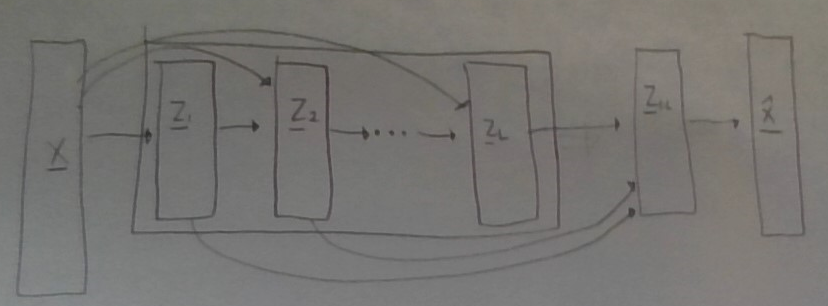
\includegraphics[width=1.0\textwidth]{Network_Illustration}
\end{figure}
As seen above, the input student data, $x$, is fed into each stochastic layer, $z_{i}$.  The stochastic layer $z_i$ has as input $x$ and $z_{i-1}$, the previous layer.  All the random variables are then taken as is to form $z_{1:L}$.  Note that nothing new happens to form  $z_{1:L}$: the random variables generated from $z_1$ to $z_L$ are each collected as is to form this layer.  No new layers or random processes happen.  \\
From here, $z_{1:L}$ is used with the Q-matrix to generate the reconstruction of the input, $\hat{x}$.  The question becomes, how does one derive $\mathcal{L}(q)$ for this new network?  To derive this, we begin a new variational lower bound identity.

%%%%%%%%%%%%%%%%%%%%%%%%%%%%%%%%%%%%%%%%%%%%%%%%%%%%%%%%%%%%%%%%%%%%%%%%%%%%%%%
%Variational Lower Bound Identity
%%%%%%%%%%%%%%%%%%%%%%%%%%%%%%%%%%%%%%%%%%%%%%%%%%%%%%%%%%%%%%%%%%%%%%%%%%%%%%%
\begin{proof}
	\begin{align*}
	logp(x) &= \mathrm{E}_{q(z_{1:L}|x)}[logp(x)] \\
	&= \mathrm{E}_{q(z_{1:L}|x)}[logp(x,z_{1:L}) - logp(z_{1:L}|x)]\\
	&= \mathrm{E}_{q(z_{1:L}|x)}[(logp(x,z_{1:L}) - logq(z_{1:L}|x)) - (logp(z_{1:L}|x)- logq(z_{1:L}|x))]\\
	&= \mathrm{E}_{q(z_{1:L}|x)}[(logp(x,z_{1:L}) - logq(z_{1:L}|x))] - \mathrm{E}_{q(z_{1:L}|x)}[logp(z_{1:L}|x)- logq(z_{1:L}|x)]\\
	&= \mathcal{L}(q) + \mathrm{KL}(q(z_{1:L}|x)||p(z_{1:L}|x))
	\end{align*}
\end{proof}
where 
\begin{equation} \label{new_LB}
\mathcal{L}(q) = \mathrm{E}_{q(z_{1:L}|x)}[(logp(x,z_{1:L}) - logq(z_{1:L}|x))]
\end{equation}
As in the previous derivation, the KL term is intractible, so we ignore it and maximize $\mathcal{L}(q)$.  Using equation (5) we can simplify $\mathcal{L}(q)$.
\begin{proof}
	\begin{align*}
	\mathcal{L}(q) &= \mathrm{E}_{q(z_{1:L}|x)}[logp(x,z_{1:L}) - logq(z_{1:L}|x)] \\
	&= -\mathrm{E}_{q(z_{1:L}|x)}[logq(z_{1:L}|x)] + \mathrm{E}_{q(z_{1:L}|x)}[logp(x,z_{1:L})]\\
	&= -\mathrm{E}_{q(z_{1:L}|x)}[log[q(z_{1}|x) \prod_{i=2}^{L}(q(z_{i}|z_{i-1},x)]] \\ &+ \mathrm{E}_{q(z_{1:L}|x)}[logp(x|z_{1:L})] + \mathrm{E}_{q(z_{1:L}|x)}[logp(z_{1:L})]\\
	&= \sum_{i=1}^{i=L}H[p(z_{i}|z_{i-1},x)] + \mathrm{E}_{q(z_{1:L}|x)}[p(x|z_{1:L})] + \mathrm{E}_{q(z_{1:L}|x)}[p(z_{1:L})]\\
	\end{align*}
\end{proof}

where 
\begin{equation} \label{Entropy}
H[p(x)] = -\mathrm{E}_{p(x)}[p(x)]
\end{equation}
 The final line of the proof is the term to be maximized by the VAE.  While the math has been done, programming this out will take some effort.
\begin{thebibliography}{14}
\bibitem{k} 
Dieng, A., Kim, Y., Rush, A., Blei, D.
\textit{ Avoiding latent variable collapse with generative skip models.}
In ICML, 2018.

\bibitem{k} 
Edwards, H. and Storkey, A. \textit{Towards a neural
statistician.} International Conference on Learning Representations (ICLR), 2017.

\bibitem{a}
Kingma, D. and Welling, M. 
\textit{ Auto-encoding variational Bayes}. 
In ICML, 2014.
 
\bibitem{e} 
Kingma, D., Rezende, D., Mohamed, S., and Welling, M. 
\textit{Semi-supervised Learning with Deep Generative Models}.  
In Neural Information Processing Systems, 2014.
 
\bibitem{k} 
Mnih, Andriy and  Karol Gregor.
\textit{Neural Variational Inference and Learning in Belief Networksl}
In AISTATS, 2014.

\bibitem{k} 
Rezende, D. J., Mohamed, S., and Wierstra, D.
\textit{Stochastic backpropagation and approximate inference in deep generative models}
In ICML, 2014.

\bibitem{k} 
Ruiz, F. J., Titsias, M., and Blei, D.
\textit{The generalized reparameterization
	gradient.}
arXiv preprint arXiv:1610.02287, 2016.
\end{thebibliography}


\end{document}